\chapter{Introducción y motivaciones}

\section{Introducción}

\begin{figure}[!htb]
	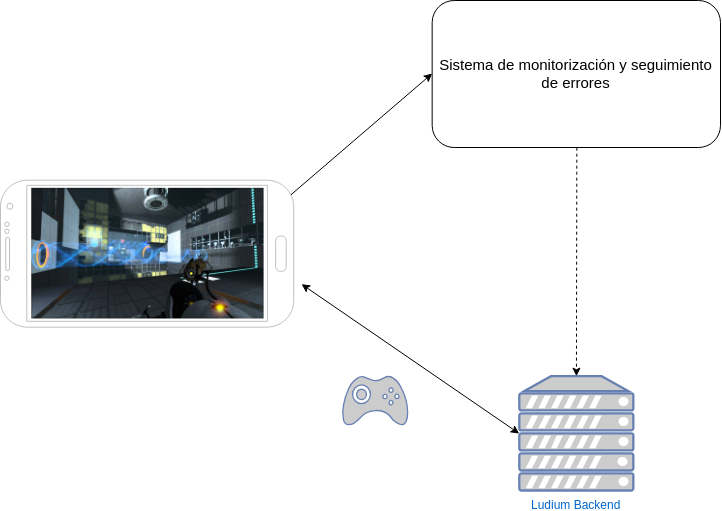
\includegraphics[width=\linewidth] {Moduloss-Intro.png}
	\caption{Visión introductoria del contexto del sistema}
	\label{fig:intro}
\end{figure}

Este proyecto es un Trabajo de Final de Grado de la modalidad B de la especialidad Tecnologías de la Información. El presente trabajo se ha hecho en colaboración con la empresa LudiumLab S.L. la cual es propietaria y creadora del servicio de cloud gaming Play Everywhere. Este servicio consiste en permitir a sus usuarios jugar a juegos diseñados para Windows PC desde otros dispositivos como podrían ser smartphones, tabletas o navegadores web. 

Dado que la empresa da servicio a dispositivos ubicuos, tiene la necesidad de recolectar y procesar eventos para que sus programadores corrijan comportamientos anómalos de la aplicación que se ejecuta en dichos dispositivos. Por lo que este trabajo es un caso de estudio para dar solución a la problemática de la empresa de recolectar y procesar eventos para darle información de valor a sus programadores.

En la Figura \ref{fig:intro} se puede ver como un dispositivo ubicuo está corriendo un videojuego diseñado para Windows PC, este videojuego realmente lo corre el Backend de Ludium y envía el video y el audio al dispositivo, el dispositivo ubicuo envía las acciones a realizar en el videojuego al Backend de Ludium. Este flujo de datos es el existente en la empresa. En la Figura \ref{fig:intro} también se ve otro flujo de datos que va del dispositivo ubicuo al Sistema de monitorización y seguimiento de errores. Este flujo de datos es el que se ha desarrollado en este trabajo. Existe un flujo de datos entre el Sistema de monitorización y seguimiento de errores, y el Backend de Ludium puesto que el sistema que se ha desarrollado se ha de integrado con ciertas partes del Backend de Ludium.

\section{Contexto}
Las aplicaciones ubicuas \cite{Tfg:ubiquitous} se han convertido ya en una constante en la vida diaria. En especial las aplicaciones dirigidas a los smartphones. Cada día aparecen nuevas aplicaciones que hacen que la informática se integre en el entorno de la persona, apareciendo en cualquier lugar y en cualquier momento. Este hecho genera nuevos retos para los desarrolladores, como pudiera ser la detección y seguimiento de errores que puedan producirse en tales aplicaciones. Las aplicaciones ubicuas hoy día pueden ejecutarse en un gran número de dispositivos. Este trabajo se centra en los smartphones y en especial en aquellos que ejecutan Android como sistema operativo.

Para controlar comportamientos anómalos en las aplicaciones, se suelen desarrollar para que, a parte de cumplir su función principal, informen sobre su estado. El registro de actividades de una aplicación es conocido como log \cite{Tfg:thelog}. Los sistemas que corren estas aplicaciones ubicuas también generan logs, en este trabajo para diferenciar los logs de las aplicaciones, de los logs del sistema, los últimos son llamados syslogs. Hay logs que directamente informan de un error y de que la aplicación ha dejado de funcionar, para diferenciar a estos logs de los syslogs y los logs, en este trabajo son llamados crashlogs. El conjunto de logs, syslogs y crashlogs es llamado alertas o eventos.

El hecho de que las aplicaciones ubicuas aparezcan en cualquier lugar y en cualquier momento, hace que muchas veces las aplicaciones ubicuas sean también aplicaciones distribuidas \cite{Tfg:distributedapp}. El controlar la comunicación y la integración de las aplicaciones con otros sistemas puede llegar a producir una cantidad de alertas (logs, syslogs y crashlogs) elevada. Al multiplicar la gran cantidad de alertas producidas por el número de instancias ejecutándose de la aplicación, se obtiene un número más que cuantioso de alertas, las cuales se han de procesar para obtener información sobre el comportamiento de las aplicaciones. Tomando el caso de Netflix\footnote{\href{https://www.netflix.com}{https://www.netflix.com}} como ejemplo \cite{Tfg:netflixpipe}, pueden llegar a generar 8 millones de eventos por segundo, lo que supone 24 GB por segundo de eventos. Por este motivo, es cada vez más frecuente entre las empresas el procesar la gran cantidad de alertas producidas por las aplicaciones con soluciones de procesado de Big Data.

Big data \cite{Tfg:bigdata} se refiere al concepto de conjuntos de datos tan masivos que las aplicaciones tradicionales de procesado de datos no son capaces de tratar con ellos. Por lo tanto, las soluciones de procesado de Big Data son todas aquellas capaces de tratar con tal volumen elevado de datos. El proceso que se suele utilizar para tratar Big Data es el de ETL (Extract, Transform and Load) \cite{Tfg:etl}, consiste en extraer los datos desde los sistemas de origen, luego transformarlos de manera oportuna y por último, una vez los datos ya han sido transformados, cargarlos en un sistema destino donde serán consumidos. 

Existen dos técnicas principales para aplicar el ETL en Big Data \cite{Tfg:batchstream}. La primera es el Batch Processing, que consiste en transformar datos que ya han estado almacenados durante un tiempo. La segunda es el Stream Processing, la cual consiste en transformar los datos en tiempo real, es decir, sin que los datos pasen mucho tiempo almacenados antes de ser transformados. 

Se encuentran dos arquitecturas de Big Data distinguidas que aplican las técnicas mencionadas. 

Una es la arquitectura Lambda \cite{Tfg:lambda}, la cual integra las dos técnicas. Consta de tres capas lógicas, una capa de Batch Processing, otra de Stream Processing y una última capa donde se sirven los datos transformados.

La otra es la arquitectura Kappa \cite{Tfg:kappa}, en la cual se utiliza únicamente Stream Processing. Consta de tres capas lógicas, una capa de Stream Processing, otra de almacenamiento persistente de datos sin transformar y una última capa donde se sirven los datos transformados.

\section{Descripción de los sistemas de alertas existentes en la empresa}
En la empresa no existía un sistema de alertas como tal, pero sí que existen servidores con software de seguimiento de incidencias y servidores de búsqueda donde almacenar los datos procesados. En concreto, el software de seguimiento de incidencias que se utiliza es JIRA\cite{Tfg:jira} y el servidor de búsqueda Elastic Search\cite{Tfg:elasticsearch}. El sistema se integra tanto con JIRA como con Elastic Search.

\section{Problema, objetivos y alcance}
\subsection{Problema}
Para que los desarrolladores puedan ofrecer la mejor experiencia de usuario necesitan recoger información de manera y forma específica sobre el comportamiento de sus aplicaciones, luego procesar esa información para poder identificar posibles comportamientos inesperados de las aplicaciones y recibir avisos con información de valor sobre los comportamientos anómalos encontrados para que puedan ser solucionados.

La empresa encuentra el problema de que esa recolección y procesado de eventos requiere de unos conocimientos sobre cómo hacer la recolección, el procesado, y que la manera y los medios que se vayan a utilizar se adapten al entorno ya existente en la empresa. Cabe destacar que no existe ningún sistema en la empresa que ya supla la necesidad de recolectar y procesar eventos, por lo que otro problema puede ser la complejidad, ya que el empezar de cero es más complejo que no aprovechar partes existentes. Otro problema se encuentra en el hecho de que la empresa tenderá a crecer y a adquirir nuevas necesidades, por lo que la escalabilidad es otro problema.

\subsection{Objetivos}
\subsubsection{Objetivo principal}
\begin{enumerate}[A)]
	\item El objetivo principal del trabajo es diseñar, implementar y desplegar un sistema que sea capaz de recolectar eventos de aplicaciones ubicuas, procesarlos e integrarse con herramientas de DevOps.
\end{enumerate}

\subsubsection{Objetivos específicos}
Para efectuar el objetivo principal, se realizarán los siguientes objetivos específicos:

\begin{enumerate}[a)]
	\item Diseño, implementación y despliegue de un protocolo para la recolección y envío de eventos (logs, syslogs y crashlogs) transparente al usuario.
	
	\item Diseño, implementación y despliegue de un sistema capaz de recibir y almacenar de forma asíncrona un volumen elevado de datos y capaz de integrarse con una herramienta de Big Data Processing.
	
	\item Configuración de una herramienta de Big Data Processing para que se integre en el sistema y almacene los datos transformados donde puedan ser consumidos.
	
	\item Integración de JIRA y Elastic Search con el sistema. Se ha de ser capaz de publicar tanto en JIRA como en Elastic Search información transformada.
\end{enumerate}


\subsection{Meta final}
Dado el tiempo limitado para realizar el Trabajo de Final de Grado, el diseño e implementación del sistema que recopile, reciba, transforme y muestre los datos, se hará lo más rápido y sencillo posible, tan solo para demostrar que la arquitectura es efectiva para el fin propuesto. La meta final se puede dividir en las siguientes metas:

\begin{enumerate}
	
	\item Una sencilla aplicación Android distribuida que genera logs, crashlogs y syslogs, y que usa una librería que de manera transparente al usuario y en el momento más oportuno, recopila eventos y los envía a un sistema para que sean procesados. 
	
	\item Un sistema, accesible por red, de recepción asíncrona y capaz de almacenar un volumen elevado de eventos, que sea escalable, resiliente a fallos en la red, independiente al dispositivo donde se ejecuta la aplicación y que se comunica con el sistema de transformación de eventos.
	
	\item Un sistema de transformación de eventos en tiempo real, siendo el núcleo del sistema una herramienta de Big Data Processing, que transforma en información útil para los desarrolladores, los datos recibidos por el sistema de recepción de eventos. Este sistema deberá almacenar en el lugar más conveniente la información transformada ya sea en JIRA o en Elastic Search. La latencia de este sistema será baja en comparación con los sistemas de Batch Processing. Las herramientas que compondrán al sistema serán modernas en la medida de lo posible. La escalabilidad del sistema ha de ser muy elevada ya que luego ha de poder ser utilizado para procesar otro tipo de datos como los derivados del Business Intelligence además unificar de todos los logs que puedan generarse en la empresa en una misma capa.
	
\end{enumerate}







\section{Estado del arte}
En esta sección se muestra el estado del arte de dos partes fundamentales del sistema. Por un lado, la recolección de eventos en Android, y por otro el procesado de eventos. Al final de la sección, se muestran las conclusiones extraídas para la creación del sistema.
\subsection{Recolección de eventos en Android}
En Android es posible ver crashlogs, syslogs o logs de aplicaciones si se trabaja conectado al dispositivo en modo depuración, este sistema para el propósito del proyecto no es útil dado que lo que se pretende es enviar tales eventos sin necesidad de conectar de forma física el dispositivo ubicuo a otro sistema. 

Existen librerías que pueden ser utilizadas para añadirle funcionalidades a las aplicaciones Android con el objetivo de que recolecten eventos y los redirijan a otros canales diferentes del estándar (el canal estándar suele ser la consola de un PC). 

Por un lado encontramos librerías especializadas en recolectar crashlogs como ACRA \cite{Tfg:acra}, que recolecta crashlogs y es capaz de redirigirlos a diferentes destinos, en esta categoría también encontramos a Breakpad \cite{Tfg:breakpad} que es un conjunto de cliente y servidor, aunque esta es más compleja de acoplar con Android.

Por otro lado encontramos librerías para generar y redirigir logs de aplicaciones. Existen librerías que tienen como base la clase Log \cite{Tfg:logclass} propia del sistema Android como es el caso de HyperLog \cite{Tfg:hyperlog}. Tales librerías suelen mejorar la clase Log consiguiendo redirigir los logs a diferentes destinos como podría ser un servidor. También encontramos librerías que no utilizan la clase Log de Android y que son propias del lenguaje Java en vez de Android. Este es el caso de las librerías basadas en log4j o su nueva versión log4j2 \cite{Tfg:log4j2}. Han habido intentos de utilizar de forma pura log4j o log4j2 en Android, pero dado que Android utiliza de manera especial ciertos aspectos de Java no se suelen utilizar de forma pura, sino que se suelen utilizar librerías adaptadas como Logback \cite{Tfg:logback} o Blitz4j \cite{Tfg:blitz4j} que se adecuan mejor a Android.

\subsection{Procesado de eventos con arquitecturas de Big Data Processing}\label{cap:procesadoBigData}
Como referencia principal en la indústria es destacable el sistema que utiliza Netflix\footnote{\href{https://www.netflix.com}{https://www.netflix.com}} para explotar sus eventos. La conocida como V2.0 Keystone pipeline \cite{Tfg:netflixpipe} utiliza una arquitectura basada en Lambda para integrar en una sola capa tanto el procesado de eventos procedentes de logs como el procesado de eventos procedentes de su BI (Business Intelligence) \cite{Tfg:bi}. Utiliza Apache Kafka \cite{Tfg:kafka}, herramienta de moda en el mundo del Big Data Processing.

Otra referencia bastante importante en la industria, es el sistema que utiliza LinkedIn\footnote{\href{https://es.linkedin.com}{https://es.linkedin.com}} para explotar los eventos que producen sus aplicaciones remotas y servidores. El conocido como Inception \cite{Tfg:inception} unifica en una sola capa todos los logs de sus dispositivos y aplicaciones para luego transformarlos y consumirlos por un software de seguimiento de errores como JIRA \cite{Tfg:jira}. Utiliza también Apache Kafka dado que el creador de dicha herramienta es trabajador de LinkedIn.

Luego es posible encontrar sistemas más enfocados al Business Intelligence pero también interesantes a considerar como es el caso de los sistemas de Spotify \cite{Tfg:spotify} o el de Twitch \cite{Tfg:twitch}. Lo destacable en el sistema de Spotify es el uso extenso de Kafka además de una integración de la capa de BI con la de logs. Lo destacable del sistema de Twitch es el modo en que hace la ingesta de datos dentro del sistema, una forma diferente con respecto a otros sistemas en la industria.

Otro sistema a destacar es el sistema de Pinterest \cite{Tfg:pinterest}, la arquitectura en sí es la clásica arquitectura Lambda sin variaciones, lo interesante de este sistema es la recolección de eventos que hace en los dispositivos, consiste en un agente (Singer \cite{Tfg:singer}) que recolecta logs en diferentes formatos y los envía a la puerta de entrada del sistema de transformación de datos, en este caso Apache Kafka.

En conclusión, encontramos que la industria lo que suele hacer para solucionar el problema de la recolección de eventos en aplicaciones ubicuas, procesado y mostrado de datos transformados es utilizar algún tipo de librería en el dispositivo ubicuo que sea capaz de recopilar los datos, y enviarlos a un agente intermedio entre el dispositivo ubicuo y el sistema de transformación de datos, una vez los datos han llegado al sistema de transformación, los datos de eventos se suelen procesar utilizando técnicas de Stream Processing. Estos sistemas de transformación de datos suelen integrar eventos y BI. Para mostrar los datos transformados suelen integrar con el sistema algún software de seguimiento de incidencias ya utilizado en la compañía y que los trabajadores ya están acostumbrados a él.

\subsubsection{Tecnologías de transformación en tiempo real}

Las tecnología expuestas en la sección \ref{cap:procesadoBigData} siguen el patrón ETL, donde la extracción es diferente para cada tipo de dispositivo al cual se le quiera extraer datos, luego tales datos se envían a un elemento intermedio (Apache Kafka) antes de transformarlos. Se puede decir que una vez los datos traspasan tal elemento intermedio empieza la transformación de los datos. Existen diferentes tecnologías con las que llevar a cabo la transformación en tiempo real, pero se van a presentar las dos más significativas y actuales.


\textbf{Apache Spark Streaming:}

Es la tecnología más popular para hacer transformaciones en tiempo real, aunque realmente no hace Stream Processing sino Micro Batching, para latencias no muy pequeñas no se diferencia el utilizar Stream Processing a Micro Batching. Es una solución ampliamente testeada y con una gran comunidad detrás, por lo que se puede encontrar bastante documentación y ejemplos, pero tiene la limitación de que realmente no hace Stream Processing. El lenguaje de implementación es en alto nivel, por lo que es bastante sencillo.

\textbf{Apache Kafka Streams:}

Es una tecnología relativamente nueva y no hace Micro Batching sino que hace un Stream Processing real. Tal solución está basada en Apache Kafka por lo que si ya se utiliza Kafka puede ser una buena opción puesto que no habrá ningún problema de integración. Una curiosidad de esta tecnología es que para procesar consume de Apache Kafka y una vez los datos han sido procesados los devuelve a Kafka, por lo que todo lo que se pueda integrar con Kafka podrá ser procesado. Aunque la documentación podría ser mayor, el lenguaje de implementación es bastante amigable y la curva de aprendizaje no es muy pronunciada.

\textbf{Logstash:}

Tanto Spark Streaming como Kafka Streams son tecnologías de propósito general, es decir, se pueden procesar todo tipo de datos ya sean eventos, mensajes o mero texto sin formatear. Existen tecnologías de propósito específico que se encargan de procesar un tipo de datos en concreto, en el caso de este proyecto el tipo de datos que interesa son los eventos (Logs, Syslogs, Crashlogs). Este es el ejemplo de Logstash parte de la ELK Stack (Logstash, Elastic Search, Kibana), que permite un procesado simple antes de almacenar los eventos.


\subsection{Procesado de eventos como servicio}
Es posible hallar empresas que ya ofrecen la solución del seguimiento y procesado de errores en las aplicaciones como un servicio, este es el caso de Crashlytics \cite{Tfg:crashlytics} o Datadog \cite{Tfg:datadog}. Existe una solución de Stream Processing como servicio de Amazon, Amazon Kinesis \cite{Tfg:kinesis}, pero no resuelve el tema de la recolección de eventos, sólo su procesado.

\subsection{Conclusiones}
Una vez analizado el estado del arte se concluye que para la recolección de eventos se utilizarán librerías ya existente y se adaptarán ciertos aspectos de estas para que se ajusten a las necesidades de la empresa, tales librerías ya implementan los requisitos buscados y se adaptan fácilmente al uso que se quiere hacer con ellas. Las librerías ACRA y Logback son buenas candidatas para ser utilizadas.

Para el procesado de eventos no se contratará ningún servicio sino que basándose en casos de uso ya existentes se diseñará, implementará y desplegará una nueva arquitectura de Big Data que se adapte a las necesidades de la empresa. No se ve conveniente contratar ningún servicio dado que es preferible ser dueño de los datos y la arquitectura para ser más flexibles a cambios en el modo de tratar los datos y el uso que se va a hacer de ellos. El uso de una arquitectura basada en el Stream Processing parece una buena aproximación para procesar los eventos, dado que tales eventos pueden contener información crítica y un procesado de baja latencia puede ayudar a corregir errores en las aplicaciones ubicuas en poco tiempo.




